\documentclass[a4paper]{article}

\usepackage[utf8]{inputenc}
\usepackage[brazil]{babel}
\usepackage{a4wide}		% correta formatacao da pagina em A4
\usepackage{setspace}		% para a distancia entre linhas
\usepackage{graphicx}
\usepackage{enumerate}

%opening
\title{Lista 2}
\author{Alisson Azzolini \and Anderson Vieira}

\begin{document}

\maketitle

\section{Caixeiro viajante}
Nesta questão, são propostas duas soluções diferentes para o problema clássico do caixeiro viajante, ambas baseadas em algoritmo genético e usando a mesma codificação, mas cada uma utilizando operadores genéticos diferentes. Na primeira implementação, é utilizado o operador de seleção roleta, e na segunda, seleção por torneio binário.

\subsection{Codificação do problema}
No problema composto por L cidades, um cromossomo é representado por uma sequência $ C = ( c_k ) $, $ c_k, k \in \{1..L\} $, onde $ c_k $ é o índice da k-ésima cidade a visitar. Como a solução é um ciclo, após a cidade $ c_L $, a cidade $ c_1 $ é revisitada.

\textsf{Exemplo} Num problema com quatro cidades, pode-se ter, por exemplo, indivíduos $ C_1 = (1, 2, 3, 4) $ e $ C_2~=~(4, 2, 3, 1) $. A representação de uma solução não é única. Assim, por exemplo, o cromossomo $ C_3~=~(1, 4, 2, 3) $ representa a mesma solução 

\subsection{Instância do problema}

A instância do problema a ser tratada é ilustrada na figura~\ref{fig:otima}. A solução-guia, obtidq a partir do site, é representada na figura. Esta solução tem comprimento de caminho $75.66$.

\begin{figure}[h!]
  \centering
  \includegraphics[scale=0.8]{optimal_trip}
  \caption{Instância \textit{Ulysses22}, com a solução ótima fornecida pelo site}
  \label{fig:otima}
\end{figure}

\subsection{Solução 1: Roleta}

A implementação da roleta é clássica. A função de fitness utilizada para a roleta é
$$
f(l) = {1 \over l}
$$
onde $ l $ é o comprimento do caminho gerado pelo indivíduo avaliado.

A população inicial $ P_{0} $ do algoritmo é formada por $ N $ indivíduos compostos de permutações aleatórias da sequência $ (1,2,\dots,L) $.

As populações $ P_{k+1} $ sucessivas, sempre de tamanho $ N $, são geradas a partir de mutações e cross-over de indivíduos selecionados a partir de $ P_{k} $ através da roleta. Os operadores de mutação e cross-over são explicados a seguir.

\subsubsection{Mutação}
Dado um indivíduo $ C_1 = (c_{1i}) $, o indivíduo mutado $ C_2 = (c_{2i}) $ consiste a aplicação de uma dentre as três operações (com $ a, b \in \{1 \dots L \}, a \leq b $ tomados aleatoreamente)
\begin{itemize}
 \item permutação pontual de cidades:

$$
c_{2i} = 
\left\{
\begin{array}{ll}
  c_{1b} & \textrm{se}~ i=a \\
  c_{1a} & \textrm{se}~ i=b \\
  c_{1i} & \textrm{c.c.} \\
\end{array}
\right.
$$

\textsf{Exemplo} $ C_1 = (1, 2, 3, 4, 5) $ muta para $ C_2 = (1, 5, 3, 4, 2) $, com $ a = 2 $ e $b = 5 $.

\item inversão de subsequências,

$$
c_{2i} = 
\left\{
\begin{array}{ll}
  c_{1(a+b-i)} & \textrm{se}~ a \leq i \leq b \\
  c_{1i} & \textrm{c.c.} \\
\end{array}
\right.
$$

\textsf{Exemplo} $ C_1 = (1, 2, 3, 4, 5) $ muta para $ C_2 = (1, 4, 3, 2, 5) $, com $ a = 2 $ e $b = 4 $.

 \item deslocamento unitário de subsequência. 

$$
c_{2i} = 
\left\{
\begin{array}{ll}
  c_{1b} & \textrm{se}~ i=a \\
  c_{1(i-1)} & \textrm{se}~ a < i \leq b \\
  c_{1i} & \textrm{c.c.} \\
\end{array}
\right.
$$

\textsf{Exemplo} $ C_1 = (1, 2, 3, 4, 5) $ muta para $ C_2 = (1, 5, 2, 3, 4) $, com $ a = 2 $ e $b = 5 $.

\end{itemize}

A escolha de qual das três operações efetuar é feita aleatoriamente, a cada mutação. Assim, o algoritmo usa os três operadores simultaneamente.

\subsubsection{Recombinação}

Foram implementadas duas recombinações diferentes, a primeira baseada na recombinação clássica e a segunda, implementando um algoritmo guloso.

A primeira recombinação consiste em uma adaptação do cross-over clássico de GA. Toma-se um pivô $ p = \{1 \dots L\} $ aleatoriamente. O indivíduo filho contém as cidades de um dos pais até $ p $ e do outro pai a partir de $ p $. As cidades repetidas são removidas uma a uma, sendo substituída por uma cidade ainda não usada, aleatoreamente.

A segunda recombinação consiste em um algoritmo guloso. Tal algoritmo monta o caminho a partir de arestas dos pais. Para cada nova cidade do filho. O algoritmo abaixo recebe como entrada dois pais, $P_1$ e $P_2$, e gera um filho $F$.

\begin{itemize}
\item  $ F \leftarrow \emptyset $
\item  $ v \leftarrow \textit{vértice aleatório} \in P_1 $
\item  $ F \leftarrow F \cup v $
\item  enquanto $ |F| < L $
\begin{itemize}
    \item $ u_1 \leftarrow \textit{próximo}(P_1, v) $
    \item $ u_2 \leftarrow \textit{próximo}(P_2, v) $
    \item $ u_{min} \leftarrow \arg\min_{u \in \{u_1, u_2\} } \textit{dist}(v, u) $
    \item $ u_{max} \leftarrow \arg\max_{u \in \{u_1, u_2\} } \textit{dist}(v, u) $
    \item 
    $
    v \leftarrow 
    \left\{
    \begin{array}{ll}
      u_{min} & \textrm{se}~ u_{min} \notin F \\
      u_{max} & \textrm{se}~ u_{min} \in F \textit{e}~ u_{max} \notin F \\
      \arg\min_{w \in P_1 - F } \textit{dist}(v, w) & \textrm{c.c.} \\
    \end{array}
    \right.
    $
    \item  $ F \leftarrow F \cup v $
\end{itemize}
\end{itemize}


\subsection{Solução 2: Torneio binário}

A população inicial $ P_{0} $do algoritmo é formada por $ N $ indivíduos compostos de permutações aleatórias da sequência $ (1,2,\dots,L) $.

Seja $ P_{k} $ o conjunto de indivíduos na geração $ k $. O operador de seleção por torneio seleciona $ m < |P_k| $ indivíduos dessa população, gerando o conjunto $ S_{k} $, da seguinte forma:

\begin{itemize}
 \item faz $ S_{k} = \emptyset $
 \item enquanto $ |S_{k}| < m $
\begin{itemize}
 \item toma indivíduos $ i_1, i_2 \in P_{k} $, aleatoriamente
 \item faz $ S_{k} = S_{k} \cup \arg\max_{\{i_1,i_2\}}\{fitness(i)\} $
\end{itemize}
\end{itemize}

Na implementação realizada, toma-se $ m = {N \over 3} $, $ N = |P_k| $.

De posse dos indivíduos selecionados na k-ésima geração, o algoritmo gera a nova população, $ P_{k+1} $, da seguinte forma:

\begin{itemize}
 \item faz $ P_{k+1} = \emptyset $
 \item enquanto $ |P_{k+1}| < N $
\begin{itemize}
 \item toma $ i_1, i_2 \in S_{k} $, aleatoriamente
 \item com probabilidade $ p_c $, recombina $ i_1 $ e $ i_2 $
 \item com probabilidade $ p_m $, muta $ i_1 $
 \item com probabilidade $ p_m $, muta $ i_2 $
 \item faz $ P_{k+1} = P_{k+1} \cup \{i_1, i_2\} $
\end{itemize}
\end{itemize}

No procedimento acima, os operadores de mutação e de recombinação são ainda os mesmos da seção anterior.

\subsection{Resultados}

\subsubsection{Roleta}
O algoritmo baseado em roleta foi rodado em dois casos: usando a recombinação clássica e a gulosa. Em ambos os casos, os seguintes parâmetros foram tomados:

\begin{eqnarray*}
p_c &=& 0.5\\
p_m &=& 0.5\\
N &=& 40\\
\textit{núm. gerações} &=& 1400
\end{eqnarray*}

No caso da seleção por roleta usando recombinação clássica, a representação do melhor indivíduo encontra-se na figura~\ref{fig:roleta_gencombine_best}, e a evolução do melhor indivíduo ao longo das gerações, na figura~\ref{fig:roleta_gencombine_evol}.

Para recombinação gulosa, a representação do melhor indivíduo encontra-se na figura~\ref{fig:roleta_greedy_best}, e a evolução do melhor indivíduo ao longo das gerações, na figura~\ref{fig:roleta_greedy_evol}.

\begin{figure}
\begin{minipage}[b]{0.5\linewidth} % A minipage that covers half the page
\centering
\includegraphics[width=8cm]{roleta_gencombine_best}
\caption{Roleta clássica: melhor obtido}
\label{fig:roleta_gencombine_best}
\end{minipage}
\hspace{0.5cm} % To get a little bit of space between the figures
\begin{minipage}[b]{0.5\linewidth}
\centering
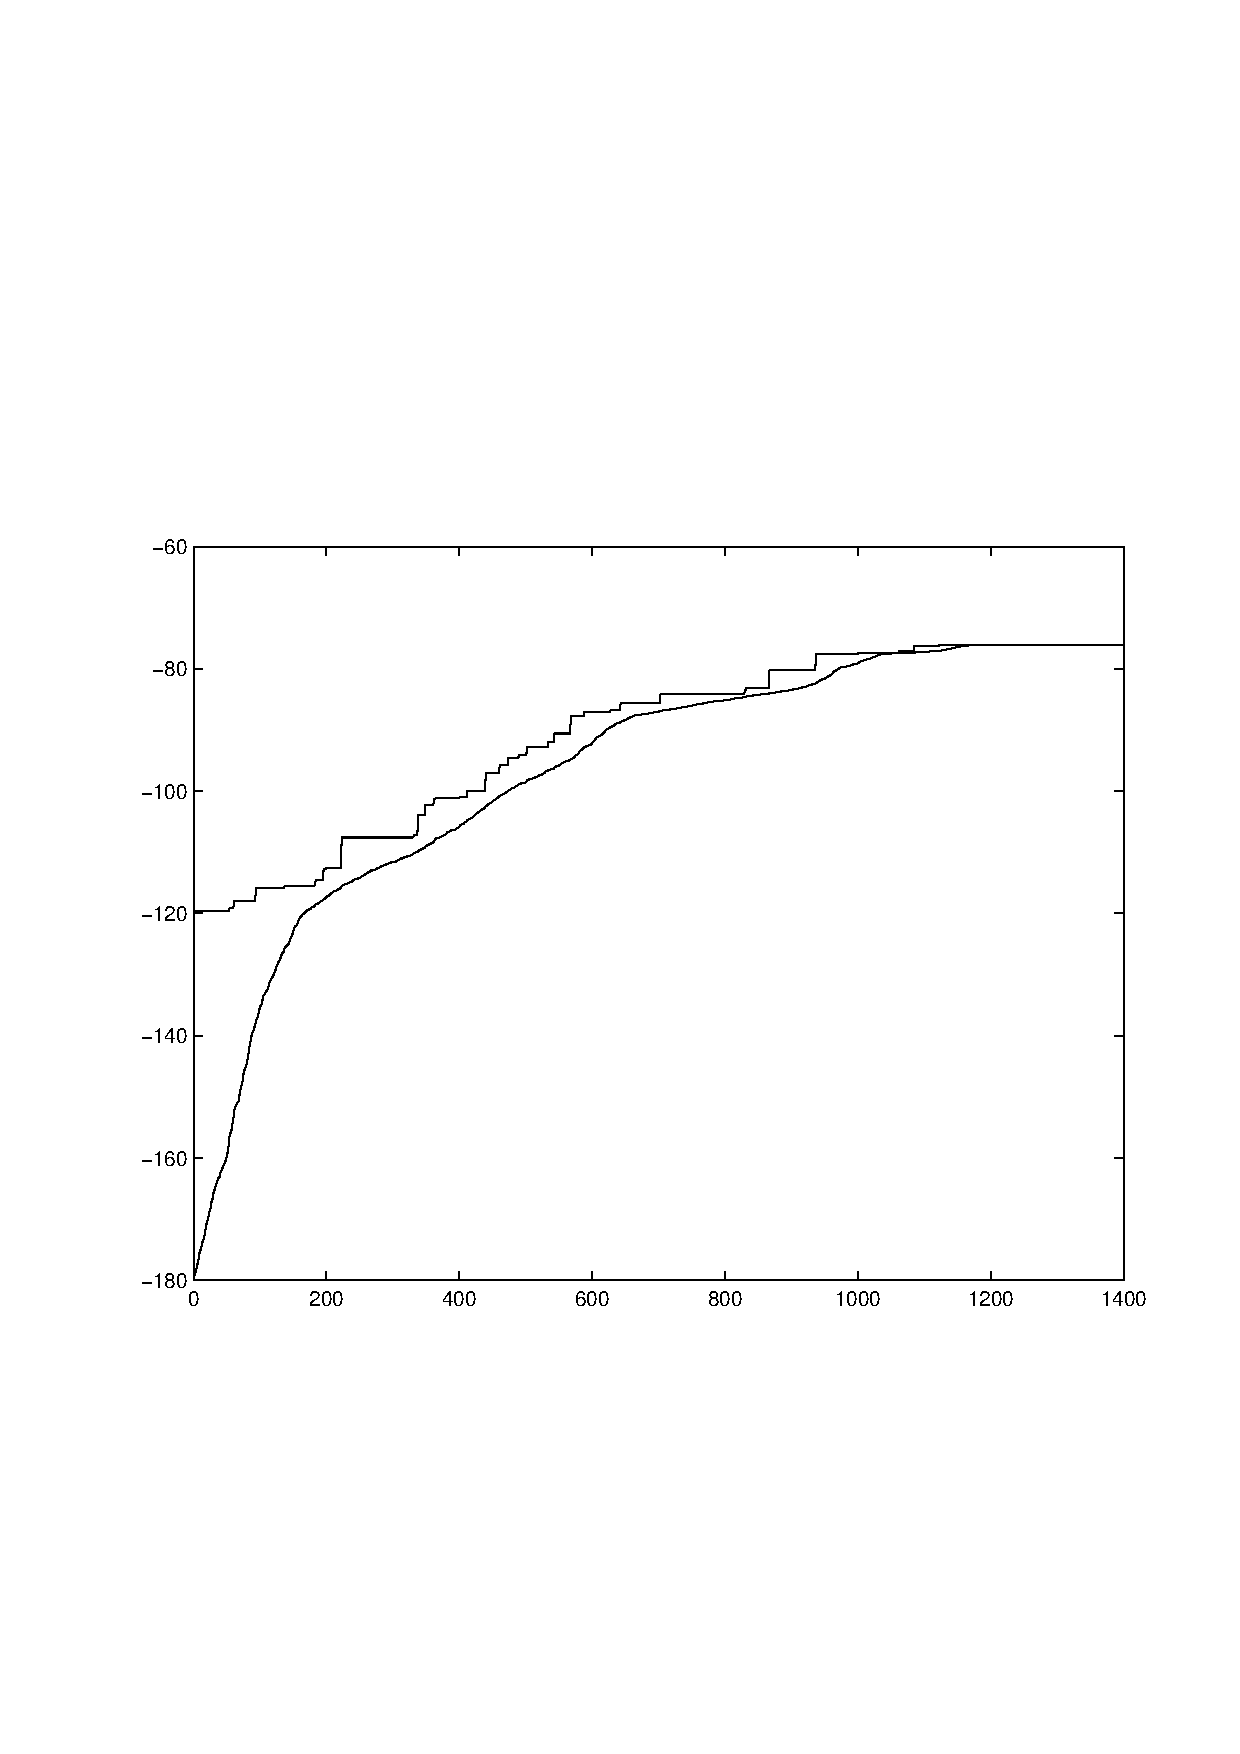
\includegraphics[width=8cm]{roleta_gencombine_evol}
\caption{Roleta clássica: evolução}
\label{fig:roleta_gencombine_evol}
\end{minipage}
\end{figure}

\begin{figure}
\begin{minipage}[b]{0.5\linewidth} % A minipage that covers half the page
\centering
\includegraphics[width=8cm]{roleta_greedy_best}
\caption{Roleta gulosa: melhor obtido}
\label{fig:roleta_greedy_best}
\end{minipage}
\hspace{0.5cm} % To get a little bit of space between the figures
\begin{minipage}[b]{0.5\linewidth}
\centering
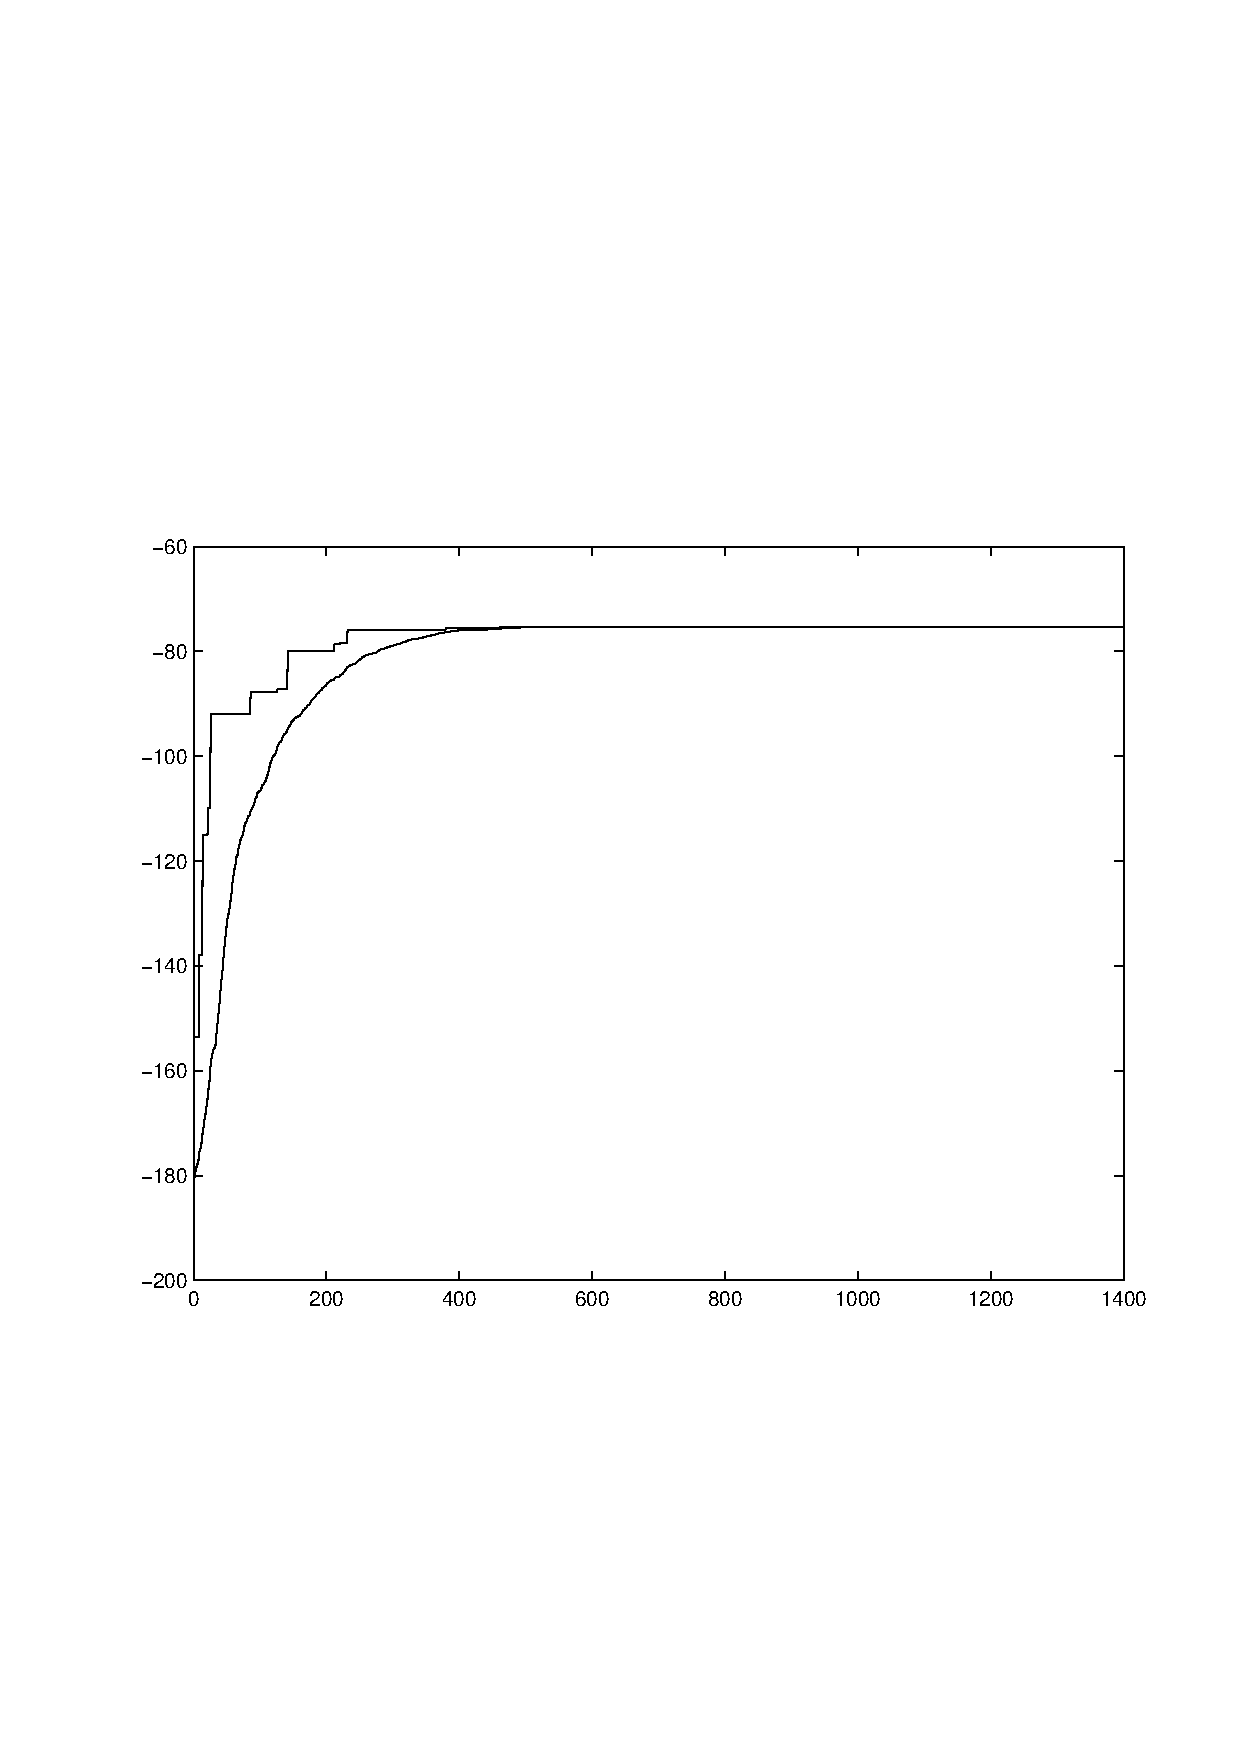
\includegraphics[width=8cm]{roleta_greedy_evol}
\caption{Roleta gulosa: evolução}
\label{fig:roleta_greedy_evol}
\end{minipage}
\end{figure}

\subsubsection{Torneio}

\begin{figure}
\begin{minipage}[b]{0.5\linewidth} % A minipage that covers half the page
\centering
\includegraphics[width=8cm]{torneio_gencombine_best}
\caption{Torneio, clássico: melhor obtido}
\label{fig:torneio_gencombine_best}
\end{minipage}
\hspace{0.5cm} % To get a little bit of space between the figures
\begin{minipage}[b]{0.5\linewidth}
\centering
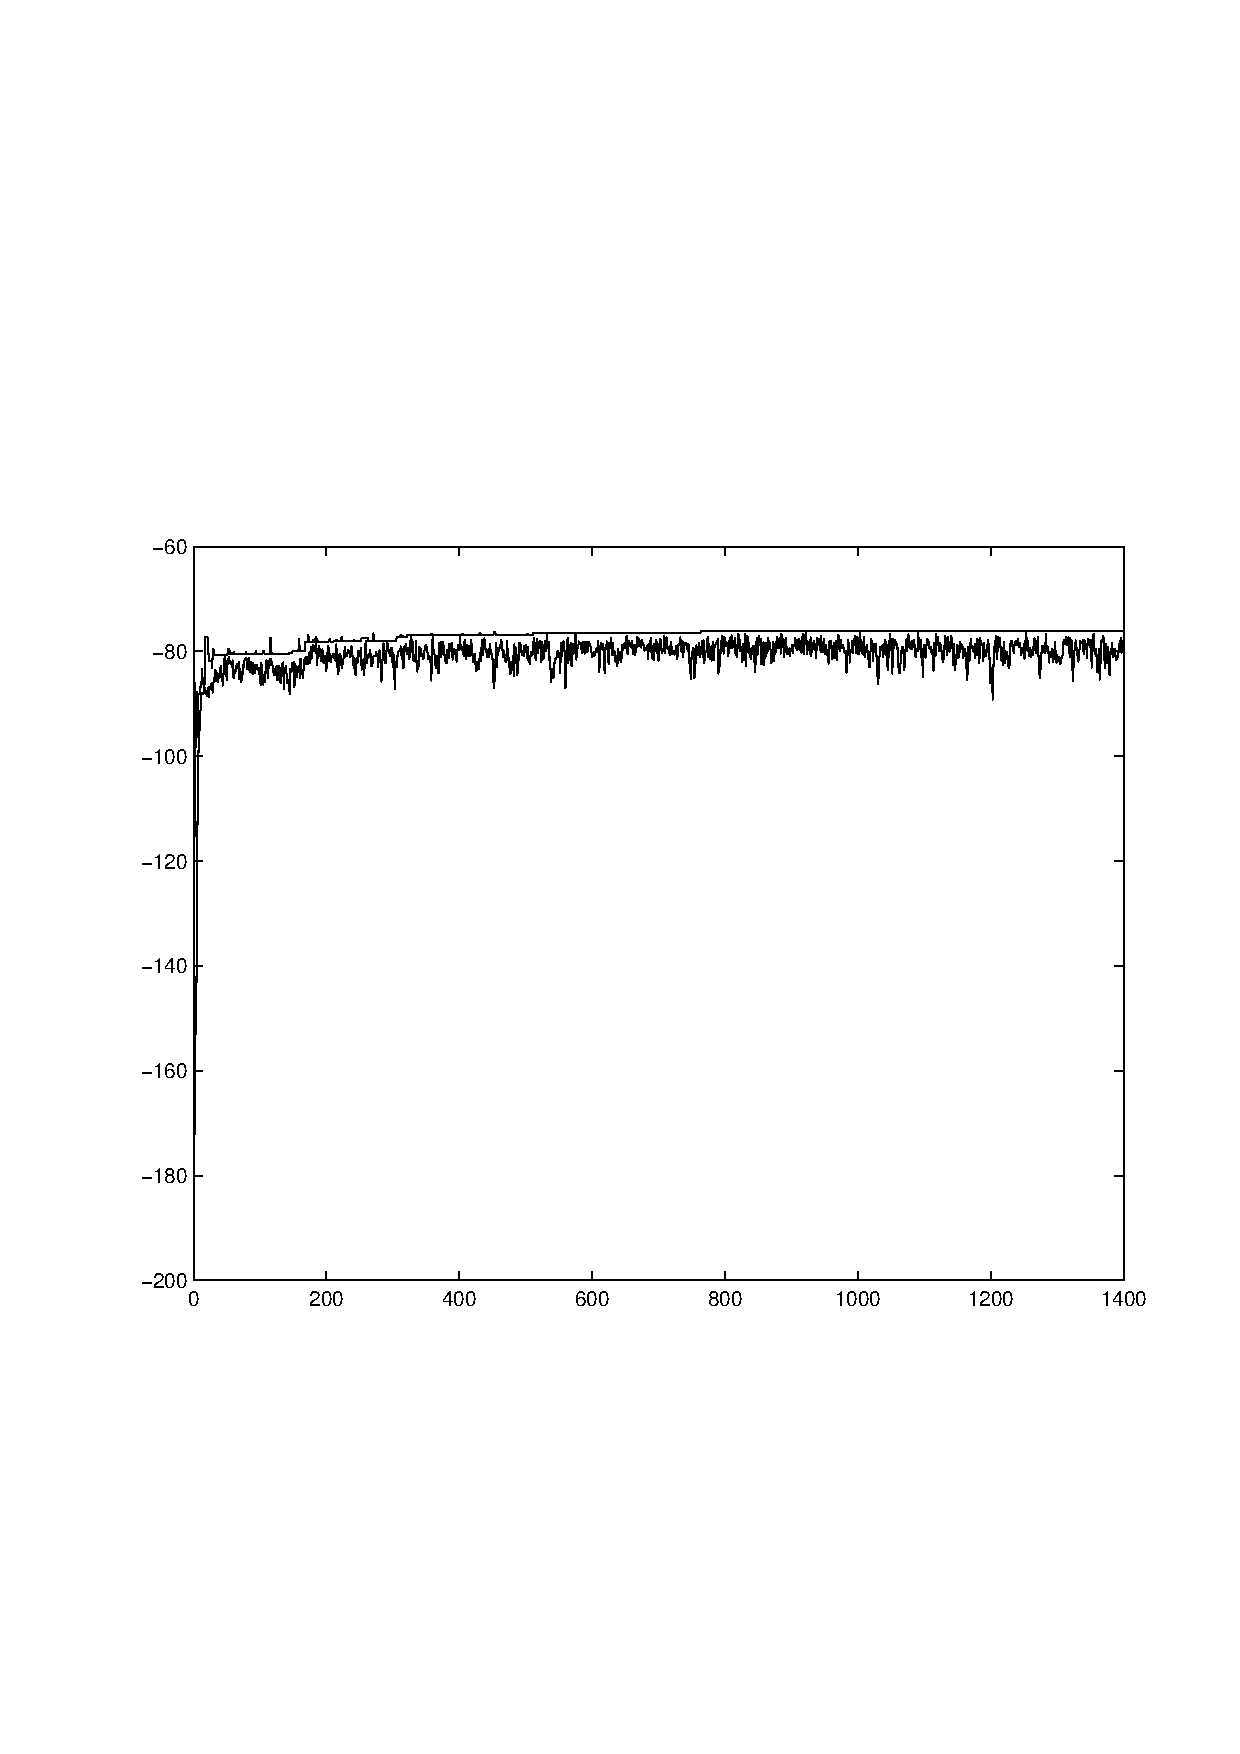
\includegraphics[width=8cm]{torneio_gencombine_evol}
\caption{Torneio, clássico: evolução}
\label{fig:torneio_gencombine_evol}
\end{minipage}
\end{figure}

\begin{figure}
\begin{minipage}[b]{0.5\linewidth} % A minipage that covers half the page
\centering
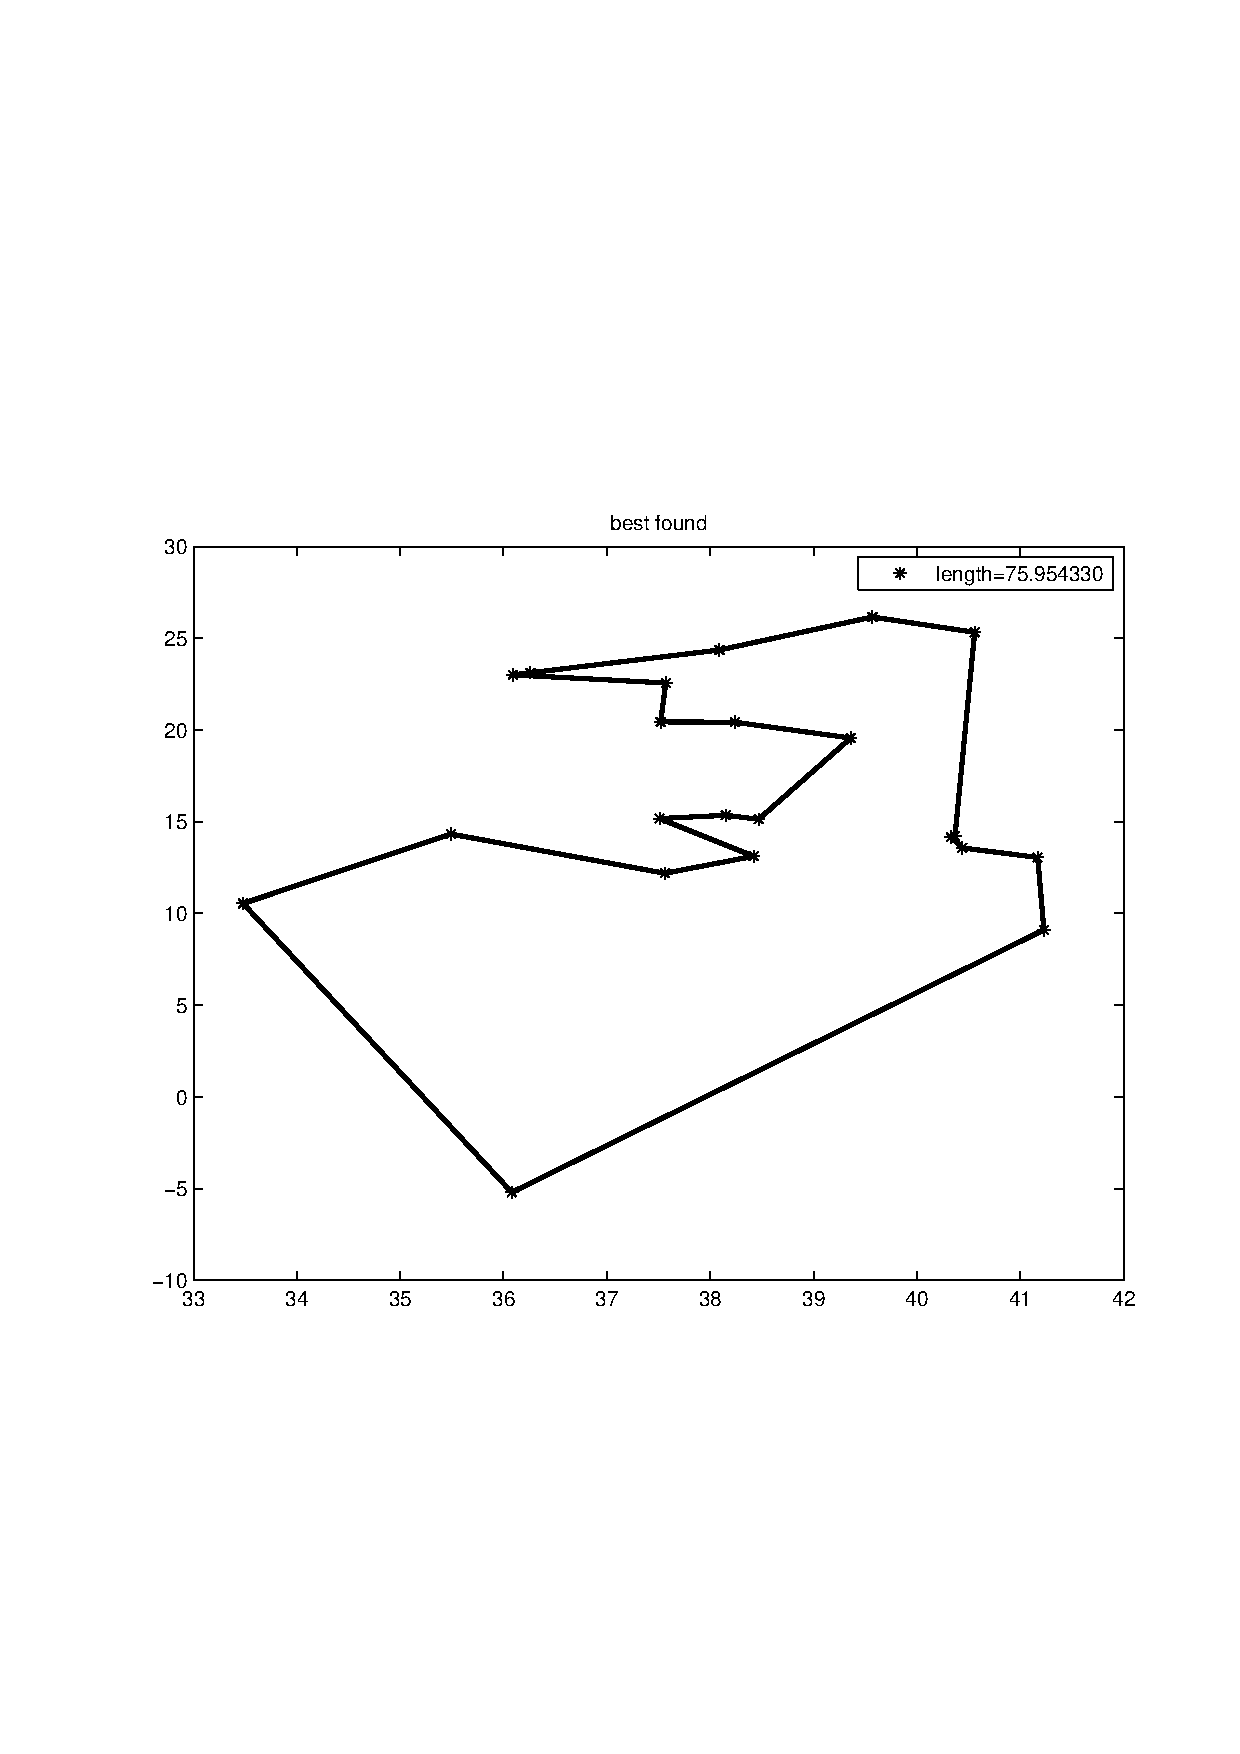
\includegraphics[width=8cm]{torneio_greedy_best}
\caption{Torneio, guloso: melhor obtido}
\label{fig:torneio_greedy_best}
\end{minipage}
\hspace{0.5cm} % To get a little bit of space between the figures
\begin{minipage}[b]{0.5\linewidth}
\centering
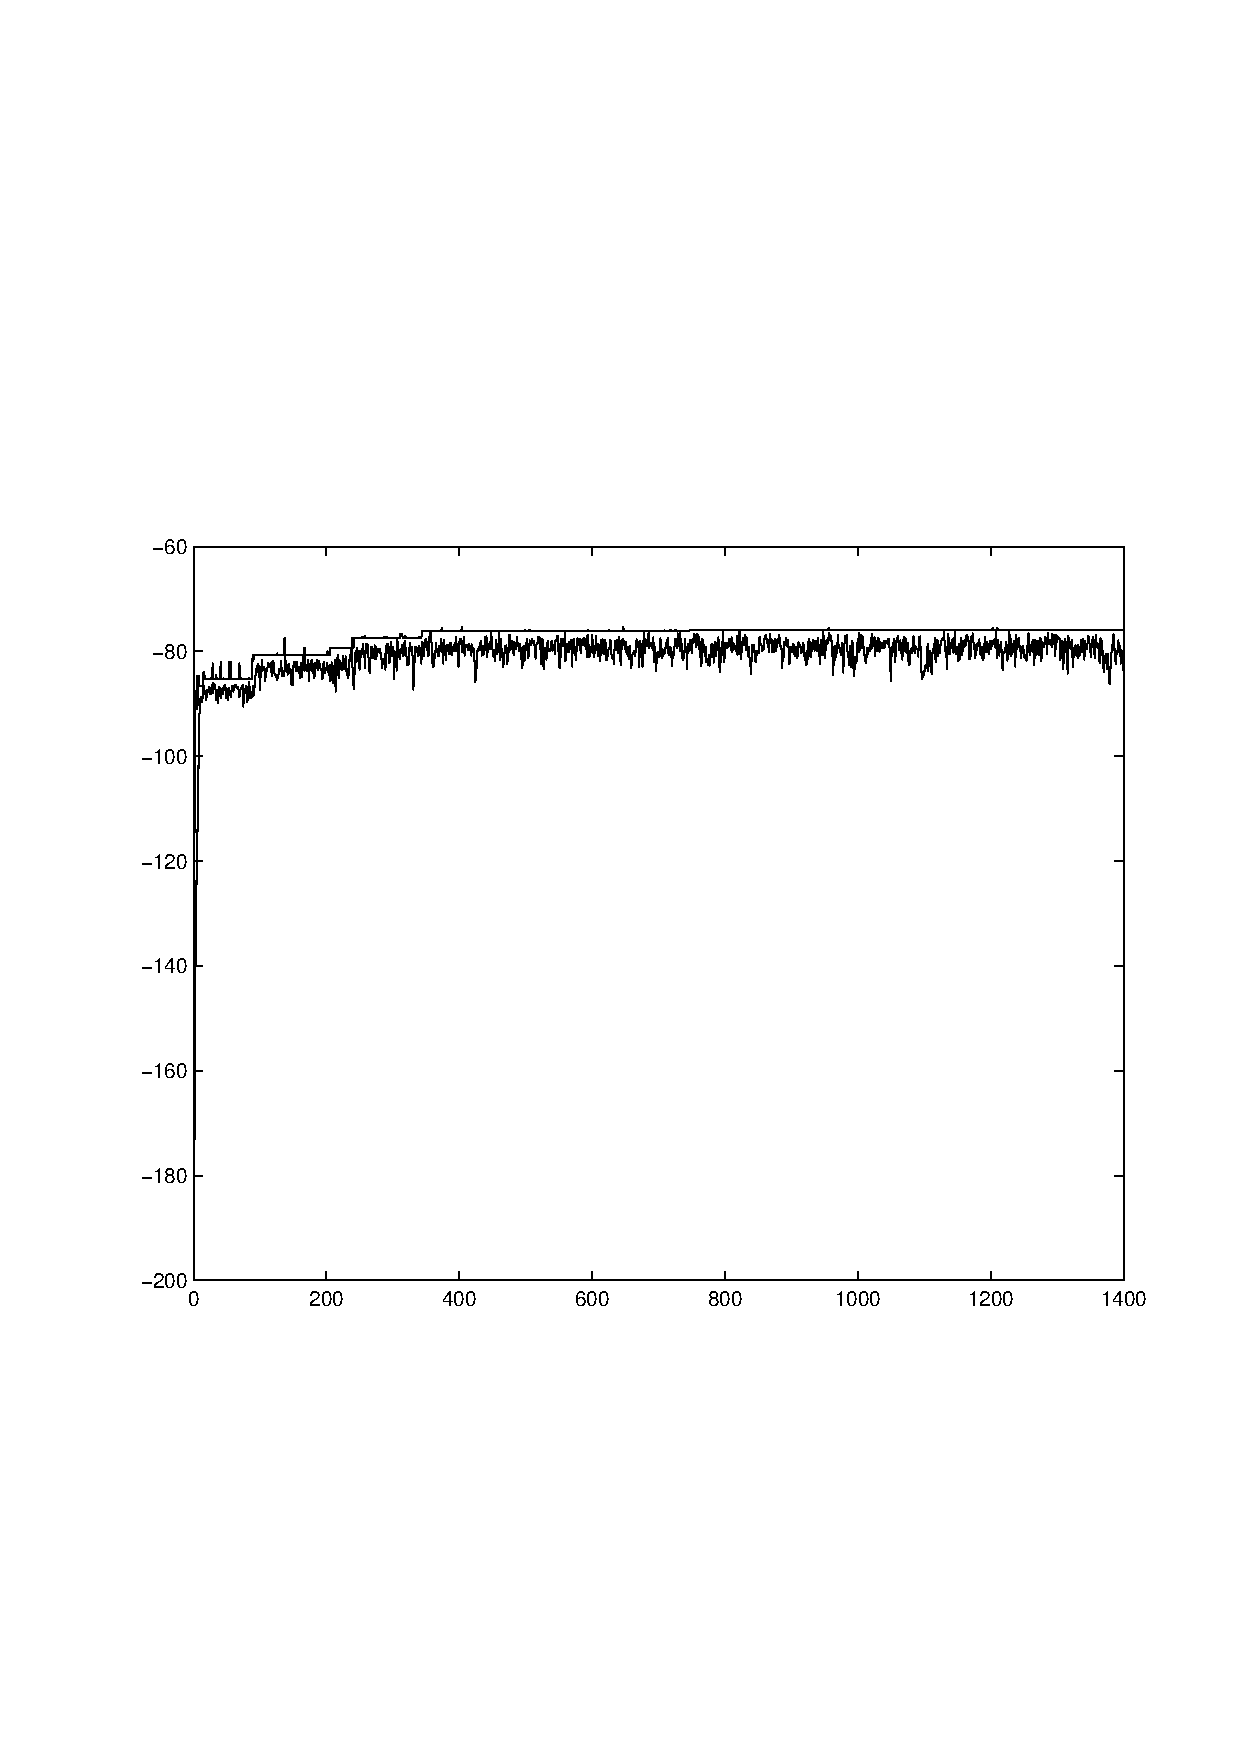
\includegraphics[width=8cm]{torneio_greedy_evol}
\caption{Torneio, guloso: evolução}
\label{fig:torneio_greedy_evol}
\end{minipage}
\end{figure}

O torneio também foi rodado com os dois operadores diferentes de cross-over, separadamente. Os parâmetros utilizados foram:

\begin{eqnarray*}
p_c &=& 0.1\\
p_m &=& 0.1\\
N &=& 40\\
\textit{núm. gerações} &=& 1400
\end{eqnarray*}

Note que, enquanto o tamanho da população $N$ e o número de gerações foram mantidos, as taxas $p_c$ e $p_m$ de cross-over e mutação foram reduzidas em relação à roleta. Tal escolha tem por objetivo compensar o aumento de oscilação do fitness causado pela redução da pressão seletiva do torneio em relação à roleta. Com taxas menores de mutação e recombinação, os indivíduos gerados são menos diferentes de geração para geração, e a pressão seletiva pode atuar ao longo de mais gerações.

Os resultados obtidos para o torneio utilizando recombinação clássica encontram-se nas figuras~\ref{fig:torneio_gencombine_best} e~\ref{fig:torneio_gencombine_evol}. Para o torneio com recombinação gulosa, os resultados estão nas figuras~\ref{fig:torneio_greedy_best} e~\ref{fig:torneio_greedy_evol}.

\subsubsection{Discussão}
Os resultados obtidos foram altamente satisfatórios, todos muito próximos, em fitness, da solução-guia apresentada na figura~\ref{fig:otima}, nenhum ultrapasando o comprimento $77$ para o caminho. Na verdade, a solução obtida pelo algoritmo com seleção roleta usando a recombinação gulosa apresentou um resultado melhor que o resultado-guia, como mostra a figura~\ref{fig:roleta_greedy_best}.

Comparando-se por exemplo as figuras~\ref{fig:roleta_greedy_evol} e~\ref{fig:torneio_greedy_evol}, nota-se que a seleção por torneio leva muito mais rapidamente a uma solução satisfatória para o problema. Na primeira dezena de iterações, o fitness da população já estava estabilizado no algoritmo do torneio. Já para a roleta, foram necessárias mais de 1000 gerações para se chegar a um fitness estável. 

Apesar disso, nota-se que mesmo depois de muitas gerações de fitness máximo estabilizado, o torneio mantém uma diversidade de fitness em sua população, comparando-se o fitness médio com o fitness máximo da população nas figura~\ref{fig:torneio_greedy_evol}. Já na roleta, a população perde rapidamente sua diversidade, e os indivíduos de uma população passam a se parecer muito com o melhor indivíduo, pelo menos quanto ao valor de fitness, como mostra a figura~\ref{fig:roleta_greedy_evol}.

Quanto à diferença de performance entre o operador de recombinação clássico e o guloso, nota-se que o guloso sempre apresentou melhores soluções, porém as diferenças de fitness ótimo foram muito pequenas (menores que 5\%). Como diferença marcante, porém, nota-se uma melhora na velocidade de convergência do algoritmo baseado em roleta quando foi usado o cross-over guloso, conforme mostram as figuras~\ref{fig:roleta_gencombine_evol} e~\ref{fig:roleta_greedy_evol}.


\section{Discussão sobre algoritmos evolutivos}
Nesta questão, discute-se a aplicabilidade e adequabilidade da solução de seis problemas distintos através de algoritmos evolutivos.

\subsection{Problema 1}
\textit{Problema com espaço de soluções contínuo e limitado, função de avaliação contínua e derivável e imagem contínua e limitada }

\textsf{Possível}, \textsf{Não recomendado}. Existem métodos de primeira e segunda ordem que tiram proveito do fato da função ser derivável e conseguem chegar rapidamente a uma solução. Um problema destes métodos porém, é que eles param ao encontrar o primeiro mínimo local. Outras heurísticas, como simulated annealing por exemplo, podem ser usadas para amenizar esta dificuldade.

\subsection{Problema 2}
\textit{Problema com espaço de soluções contínuo e limitado, função de avaliação contínua mas 
não-derivável e imagem contínua e limitada }

\textsf{Possível}, \textsf{Adequabilidade depende}. Como a função de avaliação é não-derivável métodos de primeira e segunda ordem não são aplicáveis. A prinpício não há problemas em se usar um algoritmo evolutivo, mas como o problema é bem comportado, podem existir métodos mais especializados que se saiam melhor.

\subsection{Problema 3}
\textit{Problema com espaço de soluções contínuo e limitado, função de avaliação descontínua, mas multi-modal com número finito de modos e imagem discreta }

\textsf{Possível}, \textsf{Adequabilidade depende}. Caso a função de avaliação apresente muita diferença entre indivíduos próximos no espaço de soluções, o algoritmo evolutivo se torna ineficiente. Porém, com uma boa função de avaliação, é possível atingir resultados satisfatórios. 

\subsection{Problema 4}
\textit{Problema com espaço de soluções discreto, infinito e não-limitado }

\textsf{Possível}, \textsf{Adequabilidade depende}. O fato da função de avaliação não estar especificada dificulta determinar se um algoritmo evolutivo seria uma boa abordagem. Além disso, como o espaço de solução é não limitado é muito difícil estimar um tamanho de população adequado para realizar uma boa amostragem do problema, sem comprometer o desempenho.

\subsection{Problema 5}
\textit{Problema com espaço de soluções discreto, infinito mas limitado e função de avaliação multi-modal, com número finito de modos }

\textsf{Possível}, \textsf{Recomendado}. Se o número de modos é conhecido, é possível utilizar o algoritmo evolutivo para encontrar modos iterativamente até que todos tenham sido encontrados. Caso contrário, deve-se usar um critério de parada que considere a multi-modalidade em um espaço infinito. Uma dificuldade, nesse caso, é que não se conhece, a priori, nem se pode estimar, a distância média entre ótimos de modos diferentes, já que o espaço de busca é infinito. 

\subsection{Problema 6}
\textit{Problema com espaço de soluções discreto e finito e função de avaliação multi-modal, com número finito de modos }

\textsf{Possível}, \textsf{Recomendado}. Um algoritmo evolutivo poderia encontrar boas soluções neste caso desde que usasse técnicas, como a divisão por nichos por exemplo, para encontrar os vários ótimos. Como o espaço de soluções é finito, é mais fácil determinar se uma parcela significativa do espaço de busca já foi explorada. Além disso, pode-se estimar a distância média entre os ótimos de modos diferentes (considerando uma distribuição uniforme, por exemplo).

\end{document}
 